\documentclass[12pt]{article}
\title{HW1}
\author{Maedeh Karkhaneh Yousefi}
\usepackage{graphicx}
\usepackage{float}
\usepackage{amsmath}
\usepackage{subcaption}
\usepackage{hyperref}
\hypersetup{
    colorlinks=true,
    linkcolor=blue,
    filecolor=magenta,      
    urlcolor=cyan,
    }
\begin{document}
\maketitle
The data consists of 7 columns, with titles being: 'age', 'sex', 'bmi', 'children', 'smoker', 'region', 'charges'.
It consists of 1338 rows of entries. Types include float64, int64, object. I filtered the charges between 10000 range of numbers, so that it would be easier to represent in \textit{countplots}. Therefore, the specific values of charges in the table are replaced with:$ <=10k$ , $ >10k\ \& <=20k$ ,  $>20k\ \& <=30k$ , $>30k\ \& <=40k$ and  $ >40k $.  
\begin{figure}[H]
\centering
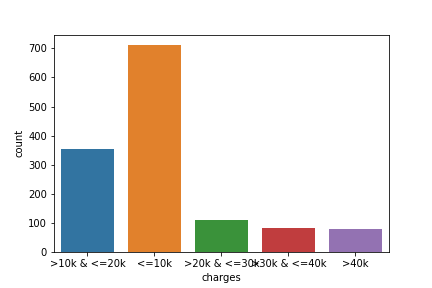
\includegraphics[width=\textwidth]{charges_dist.png}
\label{mesh:fig1}
\caption{}
\end{figure}

\begin{figure}[H]
\centering
\begin{subfigure}{0.5\textwidth}
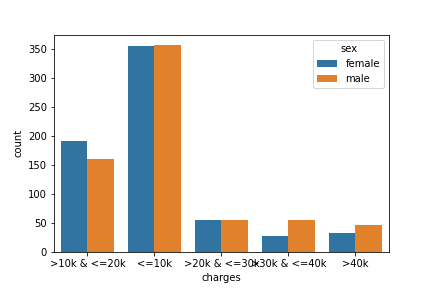
\includegraphics[width=\textwidth]{sex.png}
\end{subfigure}
\begin{subfigure}{0.5\textwidth}
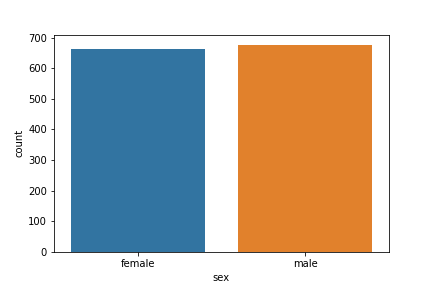
\includegraphics[width=\textwidth]{sex_dist.png}
\end{subfigure}
\label{mesh:fig1}
\caption{The number of females and males is almost equal. From the first plot it can be seen that when charges go above 30000, males have more contribution.}
\end{figure}

\begin{figure}[H]
\centering
\begin{subfigure}{0.5\textwidth}
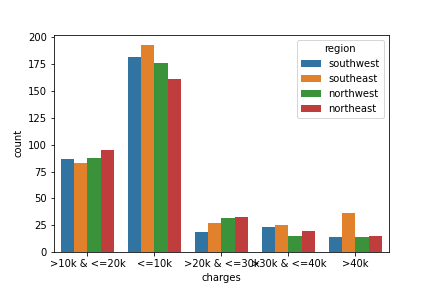
\includegraphics[width=\textwidth]{region.png}
\end{subfigure}
\begin{subfigure}{0.5\textwidth}
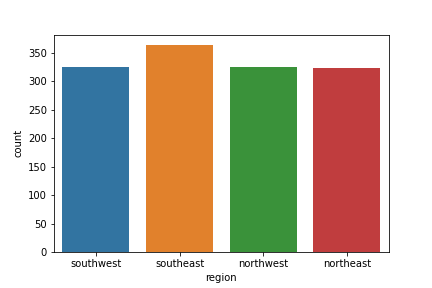
\includegraphics[width=\textwidth]{region_dist.png}
\end{subfigure}
\label{mesh:fig1}
\caption{Regions are equally distributed except for southeast, which is a little bit more than others. This could be why it has more contribution to some ranges of prices.}
\end{figure}

\begin{figure}[H]
\centering
\begin{subfigure}{0.5\textwidth}
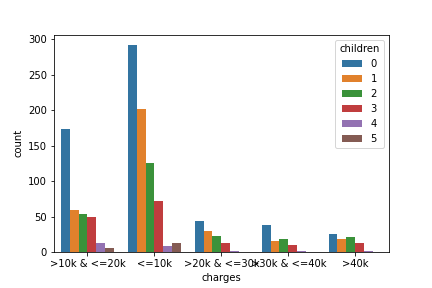
\includegraphics[width=\textwidth]{children.png}
\end{subfigure}
\begin{subfigure}{0.5\textwidth}
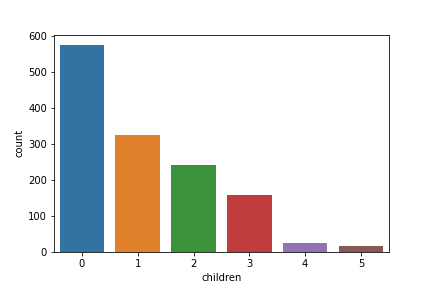
\includegraphics[width=\textwidth]{children_dist.png}
\end{subfigure}
\label{mesh:fig1}
\caption{It seems like the number of children doesn't have much effect on charges.  }
\end{figure}

\begin{figure}[H]
\centering
\begin{subfigure}{0.5\textwidth}
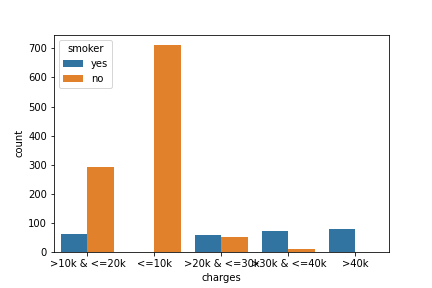
\includegraphics[width=\textwidth]{smoker.png}
\end{subfigure}
\begin{subfigure}{0.5\textwidth}
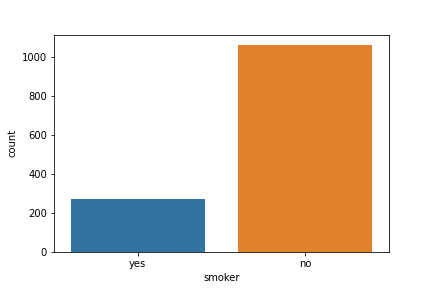
\includegraphics[width=\textwidth]{smoker_dist.png}
\end{subfigure}
\label{mesh:fig1}
\caption{From plots we can conclude that being an smoker results in higher charges.}
\end{figure}\textit{•}
\begin{center}
You can access the code by clicking \href{https://github.com/narges8k/MachineLearningWorkshop/tree/main/HW1}{here}.
\end{center}
\end{document}